% ****** Start of file apssamp.tex ******
%
%   This file is part of the APS files in the REVTeX 4.2 distribution.
%   Version 4.2a of REVTeX, December 2014
%
%   Copyright (c) 2014 The American Physical Society.
%
%   See the REVTeX 4 README file for restrictions and more information.
%
% TeX'ing this file requires that you have AMS-LaTeX 2.0 installed
% as well as the rest of the prerequisites for REVTeX 4.2
%
% See the REVTeX 4 README file
% It also requires running BibTeX. The commands are as follows:
%
%  1)  latex apssamp.tex
%  2)  bibtex apssamp
%  3)  latex apssamp.tex
%  4)  latex apssamp.tex
%
\documentclass[%
 preprint, linenumbers,
%superscriptaddress,
%groupedaddress,
%unsortedaddress,
%runinaddress,
%frontmatterverbose, 
%preprint,
%preprintnumbers,
%nofootinbib,
%nobibnotes,
%bibnotes,
 amsmath,amssymb,
 aps, physrev,
%pra,
%prb,
%rmp,
%prstab,
%prstper,
%floatfix,
]{revtex4-2}
\setlength{\parindent}{0pt}
\usepackage{graphicx}% Include figure files
\usepackage{dcolumn}% Align table columns on decimal point
\usepackage{bm}% bold math
\usepackage{subcaption}
%\usepackage{hyperref}% add hypertext capabilities
%\usepackage[mathlines]{lineno}% Enable numbering of text and display math
%\linenumbers\relax % Commence numbering lines

%\usepackage[showframe,%Uncomment any one of the following lines to test 
%%scale=0.7, marginratio={1:1, 2:3}, ignoreall,% default settings
%%text={7in,10in},centering,
%%margin=1.5in,
%%total={6.5in,8.75in}, top=1.2in, left=0.9in, includefoot,
%%height=10in,a5paper,hmargin={3cm,0.8in},
%]{geometry}
\usepackage[utf8]{inputenc} % Para caracteres especiales
\usepackage{lipsum} % Para texto de ejemplo
\usepackage{graphicx}  % Para incluir gráficos
\usepackage{float} 

\begin{document}

\preprint{APS/123-QED}

\title{\textbf{Density Functional Theory}}


\author{Jhon Fredy Gelvez Parada}
\affiliation{Physical Departament, University of Pamplona }
\date{16 de diciembre de 2024}

\date{\today}% It is always \today, today,
             %  but any date may be explicitly specified

\begin{abstract}
\noindent This article examines the foundational principles of Density Functional Theory (DFT), introduced by Hohenberg and Kohn in 1964. They proved that the electron density \(n(r)\) uniquely determines all properties of a system of interacting electrons under an external potential \(v(r)\). By defining a universal functional \(F[n]\), they showed that the ground-state energy can be obtained without requiring the full many-body wavefunction. This breakthrough transformed the study of many-electron systems, paving the way for advances in computational physics and quantum chemistry.
\end{abstract}

%\keywords{Suggested keywords}%Use showkeys class option if keyword
                              %display desired


%\tableofcontents
\maketitle
\section{\label{sec:level1}INTRODUCTION }
Density Functional Theory (DFT) is a fundamental tool in modern physics and chemistry for studying many-body systems. In 1964, Hohenberg and Kohn published a paper that marked a turning point in this field by demonstrating that the ground-state electron density, \( n_0(r) \), can be used as the basic variable to describe all properties of an interacting quantum electron system. This discovery greatly simplified the many-body problem, as it allowed reducing the complexity of working with high-dimensional wavefunctions to working with a scalar function of three spatial variables.

The work of Hohenberg and Kohn is based on two fundamental theorems. The first establishes that, for a system of electrons in an external potential \( v(r) \), there exists an energy functional \( E[n] \) that reaches its minimum value at the exact ground-state electron density. The second theorem proves that this functional is unique, meaning that the electron density contains all the necessary information to describe the system. However, while these results are theoretically elegant, they do not provide practical guidance for constructing exact functionals, which remains one of the greatest challenges in DFT.

To overcome this limitation, Kohn and Sham proposed a practical approach in 1965 that has been key to the success of DFT. Their method introduces an auxiliary system of independent particles, where the effects of electron-electron interaction are incorporated into an exchange-correlation functional. This approach has led to the development of useful approximations, such as the Local Density Approximation (LDA) and the Generalized Gradient Approximation (GGA), which have proven effective in a wide variety of applications.

Today, DFT is one of the most widely used methodologies for calculating the electronic structure of atoms, molecules, and solids. Its ability to balance accuracy with computational efficiency has made it an essential tool in condensed matter physics and computational chemistry. Moreover, its success has inspired the development of new approximations and extensions aimed at improving its accuracy and expanding its applicability.
\section{\label{sec:level1}HOHENBERG AND KOHN THEOREMS }

Density Functional Theory (DFT) is based on two fundamental theorems developed by Hohenberg and Kohn, which simplify the complex problem of describing a system of many interacting electrons. The main idea is that all the information about the system can be obtained from the electronic density distribution in its ground state.

To understand this better, imagine a system of electrons moving under the influence of an external potential \( V_{\text{ext}}(r) \). The Hamiltonian, which represents the total energy of the system, can be written as:

\begin{equation}
\hat{H} = -\frac{\hbar^2}{2m_e} \sum_i \nabla_i^2 + \sum_i V_{\text{ext}}(r_i) + \frac{1}{2} \sum_{i \neq j} \frac{e^2}{|r_i - r_j|}
\end{equation}

This equation combines three terms: the kinetic energy of the electrons, the interaction of the electrons with the external potential, and the repulsion between them due to their electric charge. The wavefunction of the ground state \( \Psi_0 \), associated with this minimum energy, has a corresponding electronic density \( n_0(r) \).

The first theorem establishes something surprising: the electronic density of the ground state completely determines the external potential \( V_{\text{ext}}(r) \), except for a constant. In other words, if we know how the electrons are distributed in space, we can know what kind of external force is affecting them.

To prove this, assume that there are two different external potentials, \( V_{\text{ext}}^{(1)}(r) \) and \( V_{\text{ext}}^{(2)}(r) \), that generate the same electronic density \( n_0(r) \). This would mean that there are two different wavefunctions \( \Psi^{(1)} \) and \( \Psi^{(2)} \), each associated with a distinct ground state with energies \( E^{(1)} \) and \( E^{(2)} \).  

Applying the principle of minimum energy, we have:

\begin{equation}
E^{(1)} = \langle \Psi^{(1)} | \hat{H}^{(1)} | \Psi^{(1)} \rangle < \langle \Psi^{(2)} | \hat{H}^{(1)} | \Psi^{(2)} \rangle
\end{equation}

Expanding this last term using the second Hamiltonian:

\begin{equation}
E^{(1)} < E^{(2)} + \int \left[V_{\text{ext}}^{(1)}(r) - V_{\text{ext}}^{(2)}(r) \right] n_0(r) \, d^3r
\end{equation}

If we perform the same calculation but swap the roles of the potentials, we obtain:

\begin{equation}
E^{(2)} < E^{(1)} + \int \left[V_{\text{ext}}^{(2)}(r) - V_{\text{ext}}^{(1)}(r)\right] n_0(r) \, d^3r
\end{equation}

Adding both expressions leads to a contradiction:

\begin{equation}
E^{(1)} + E^{(2)} < E^{(1)} + E^{(2)}
\end{equation}

This proves that there cannot be two different potentials that generate exactly the same electronic density, meaning that the external potential is completely determined by \( n_0(r) \).

The second theorem is equally important: it states that there exists a universal functional that relates the total energy \( E[n] \) to the electronic density \( n(r) \). The remarkable thing about this theorem is that the density that minimizes this functional is exactly the ground state density \( n_0(r) \). This means that, in theory, if we knew this universal functional, we could directly find the energy and the density of the system without solving the complicated Schrödinger equation.

However, the Hohenberg and Kohn theorems do not tell us how to construct this functional. Therefore, research in DFT focuses on finding practical approximations that allow us to calculate the energy of real systems. Despite this limitation, these theorems provide the theoretical foundations for one of the most powerful tools in quantum chemistry and condensed matter physics. 

The second theorem of Hohenberg and Kohn states that there exists a universal functional of the electronic density that allows calculating the total energy of an electron system subject to an external potential. Simply put, this means that by knowing how the electron density varies in space, it is possible to find the minimum energy of the system without having to solve the complicated Schrödinger equation for multiple electrons.

To better understand this, it is important to grasp the concept of a "functional" of the density. A functional is a mathematical expression that takes the electronic density \( n(r) \) as input and returns a specific quantity, such as kinetic energy or interaction energy between electrons. The theorem applies only to "V-representable" densities, i.e., those that can be generated from some external potential \( V_{\text{ext}}(r) \). This defines a space of possible densities within which these functionals can be constructed.

The total energy of the system is expressed as:

\begin{equation}
E[n] = T[n] + E_{\text{int}}[n] + \int V_{\text{ext}}(r)n(r) \, d^3r + E_{\text{II}}
\end{equation}

In this equation, \( T[n] \) represents the kinetic energy of the electrons, \( E_{\text{int}}[n] \) is the interaction energy between them, and \( E_{\text{II}} \) is the interaction energy between the nuclei. To simplify this expression, we combine the first two terms and define a universal functional:

\begin{equation}
F_{\text{HK}}[n] = T[n] + E_{\text{int}}[n]
\end{equation}

Then, the total energy becomes:

\begin{equation}
E[n] = F_{\text{HK}}[n] + \int V_{\text{ext}}(r)n(r) \, d^3r + E_{\text{II}}
\end{equation}

Now, to prove this theorem, assume there exists a ground state density \( n^{(1)}(r) \), associated with a specific external potential \( V_{\text{ext}}^{(1)}(r) \). The corresponding total energy would be:

\begin{equation}
E^{(1)} = \langle \Psi^{(1)} | \hat{H}^{(1)} | \Psi^{(1)} \rangle
\end{equation}

Now imagine another distinct density \( n^{(2)}(r) \), with a different wavefunction \( \Psi^{(2)} \). According to the principle of minimum energy, the energy associated with the correct density will always be lower than that of any other possible density:

\begin{equation}
E^{(1)} < \langle \Psi^{(2)} | \hat{H}^{(1)} | \Psi^{(2)} \rangle = E^{(2)}
\end{equation}

This proves that the total energy calculated with the Hohenberg and Kohn functional is always minimized when the correct ground state density is used.

In conclusion, if the exact functional \( F_{\text{HK}}[n] \) were known, we could find the minimum energy by simply searching for the density that minimizes the total energy. In this way, the problem could be solved without the need to calculate the wavefunction of the electrons. However, this functional provides information only about the ground state, not about excited states, which completes the proof of the second Hohenberg and Kohn theorem.

\section{\label{sec:level1}The Variational Principle }

The variational principle is a fundamental concept in Density Functional Theory (DFT) that helps us calculate the ground-state energy of an electron system. This principle is based on the idea that we can find the minimum energy of a system by minimizing a functional that depends on the electronic density \( n(r) \).

For an electron system interacting under an external potential \( v(r) \), the total energy can be expressed as:

\begin{equation}
E_v[n] = \int v(r) n(r) \, dr + F[n],
\end{equation}

where \( v(r) \) is the external potential acting on the electrons and \( F[n] \) is a universal functional that includes the kinetic energy and the interaction energy between the electrons. This functional does not depend on the external potential.

The functional \( F[n] \) can be decomposed into two parts:

\begin{equation}
F[n] = T[n] + U[n],
\end{equation}

where \( T[n] \) is the kinetic energy of the electrons and \( U[n] \) is the interaction energy between them.

The variational principle tells us that the energy functional \( E_v[n] \) reaches its minimum value when \( n(r) \) is the electronic density of the ground state. This means that:

\begin{equation}
E_v[n] \geq E,
\end{equation}

where \( E \) is the ground-state energy. Equality holds only when \( n(r) \) is the correct density.

For the minimization of \( E_v[n] \) to be valid, we must ensure that the electronic density \( n(r) \) satisfies the normalization condition, which states that the integral of the density must equal the total number of electrons \( N \):

\begin{equation}
N[n] = \int n(r) \, dr = N.
\end{equation}

In DFT, the electronic density \( n(r) \) becomes the main variable, replacing the wave function \( \Psi \). For a system of \( N \) particles, the total energy can also be expressed in terms of the wave function as:

\begin{equation}
E[\Psi] = \langle \Psi | \hat{T} + \hat{U} + \hat{V} | \Psi \rangle,
\end{equation}

where \( \hat{T} \) is the kinetic energy operator, \( \hat{U} \) is the interaction operator, and \( \hat{V} \) is the external potential operator. The wave function of the ground state minimizes this energy functional while keeping the number of particles constant.

Hohenberg and Kohn demonstrated that the external potential \( v(r) \) is unique for a given electronic density \( n(r) \), except for an additive constant. This means that if we have two different potentials that produce the same density, they cannot correspond to the same ground state.

The variational principle is crucial because it simplifies the many-body problem by focusing on the electronic density \( n(r) \) instead of the wave function \( \Psi \). This significantly reduces the complexity of the problem, as \( n(r) \) depends on only three spatial coordinates, while \( \Psi \) depends on \( 3N \) coordinates for a system of \( N \) particles.

Moreover, this principle ensures that any approximation to the functional \( F[n] \) used to calculate the energy of the system will be greater than or equal to the exact energy. This provides a solid foundation for developing practical methods in DFT, such as exchange-correlation functionals.

\section{\label{sec:level1}Transformation of the Functional \( F[n] \) }

In Density Functional Theory (DFT), the Coulomb interaction has a long-range nature, making it convenient to separate the Coulomb energy part from the functional \( F[n] \). In this context, the classical Coulomb energy \( F[n] \) is expressed as:

\begin{equation}
F[n] = \int \frac{1}{2} \frac{n(r) n(r')}{|r - r'|} \, dr \, dr' + G[n],
\end{equation}

where \( n(r) \) is the electronic density at point \( r \), and the integral represents the Coulomb interaction between all pairs of points \( r \) and \( r' \). The function \( G[n] \) is an additional term representing other components of the functional that do not directly depend on the Coulomb interaction.

From the definition of \( F[n] \) in equation (9), we can write the total energy \( E_v[n] \) of the system as:

\begin{equation}
E_v[n] = \int v(r) n(r) \, dr + \int \frac{n(r) n(r')}{|r - r'|} \, dr \, dr' + G[n],
\end{equation}

where \( v(r) \) is the external potential acting on the electrons. The first integral represents the interaction between the electrons and the external potential, while the second integral is the contribution of the Coulomb energy between the electrons. The term \( G[n] \) remains a universal functional capturing more complex effects, such as the correlation between electrons.

Now, we can analyze the expression for \( G[n] \) in more detail. Starting from the definitions of \( F[n] \) and \( G[n] \) in the previous equations, we obtain:

\begin{equation}
G[n] = \frac{1}{2} \int \left( \nabla_r \nabla_{r'} n_1(r, r') \right)_{r=r'} \, dr \, dr' + \frac{1}{2} \int C_2(r, r') \, dr \, dr',
\end{equation}

where:

\begin{itemize}
    \item \( n_1(r, r') \) is the single-particle density matrix, which describes the distribution of the electrons in the system in terms of spatial coordinates \( r \) and \( r' \).
    \item \( C_2(r, r') \) is the two-particle correlation function, which captures the effects of the interaction between two electrons. This function is defined as the difference between the density of two particles \( n_2(r, r') \) and the product of the densities of one particle \( n_1(r) n_1(r') \), that is:
\end{itemize}

\begin{equation}
C_2(r, r') = n_2(r, r'; r, r') - n_1(r) n_1(r').
\end{equation}

It is important to note that, in the case where \( r = r' \), the function \( n_2(r, r) \) reduces to \( n_1(r) \), as the density of two particles at the same point is equal to the density of one particle.

From equation (16), we can define an energy density functional that involves the density matrices and the correlation function of the particles. This functional is given by:

\begin{equation}
g_r[n] = \frac{1}{2} \left( \nabla_r \nabla_{r'} n_1(r, r') \right)_{r=r'} + \frac{1}{2} \int C_2(r - r') \left( \frac{r + r'}{2} \right) \, dr',
\end{equation}

where the first part of the equation describes the gradient of the single-particle density matrix evaluated at the same point (\( r = r' \)). The second part of the integral involves the correlation function \( C_2(r - r') \), which depends on the difference between the points \( r \) and \( r' \), weighted by the average of the positions.

Finally, we can obtain the functional \( G[n] \) by integrating \( g_r[n] \) over all space:

\begin{equation}
G[n] = \int g_r[n] \, dr.
\end{equation}

This functional \( G[n] \) is a crucial component in the calculation of the system's energy, and its correct determination is key to obtaining an accurate description of interacting electron systems in Density Functional Theory.

\section{\textbf{THE GAS OF ALMOST CONSTANT DENSITY}}

In the study of an electron gas with almost constant density, the system is described through small perturbations over a uniform density. This approach allows the application of density functional theory tools to analyze the interaction and response of the system to external perturbations.

The electron density \( n(r) \) is expressed as a perturbation over a uniform density \( n_p \), i.e.:

\begin{equation}
n(r) = n_0 + \tilde{n}(r)
\end{equation}

where \( \tilde{n}(r) \) represents a small variation. This treatment converts the system into a uniform gas with small deviations that can be approximated. To ensure that the perturbations do not alter the total number of particles, the particle conservation condition must be satisfied:

\begin{equation}
\int \tilde{n}(r) \, dr = 0
\end{equation}

In this way, the energy functional \( G[n] \) is defined, which includes both electronic interactions and other relevant contributions. The expansion of this functional in terms of \( \tilde{n}(r) \) is shown in the following equation:

\begin{equation}
G[n] = G[n_0] + \int K(r - r') \, \tilde{n}(r) \, \tilde{n}(r') \, dr \, dr'
\end{equation}

\begin{equation}
    + \int L(r, r', r'') \, \tilde{n}(r) \, \tilde{n}(r') \, \tilde{n}(r'') \, dr \, dr' \, dr'' + \dots
\end{equation}

which allows studying the behavior of the system in the presence of these small perturbations.

Additionally, the kernel \( \alpha(q) \) is introduced, which is essential to understanding the system's response to external perturbations. This kernel is related to the electronic polarizability \( n(q) \), which describes how the electron density responds to an external field. In this context, the equation

\begin{equation}
K(q) = 2\pi \left[ -c_2 + (c_2^2 - c_4)q^2 + \dots \right] \quad \text{as} \quad q \to 0
\end{equation}

indicates that \( K(q) \) has a singularity at \( q = 2k_F \), which is linked to the Friedel oscillations. This quantum phenomenon leads to periodic variations in the electron density due to the system's structure, which cannot be adequately described by classical methods such as Thomas-Fermi. Equation (49) describes how these oscillations manifest in real space, with an oscillatory term that decays slowly with distance.

The equation

\begin{equation}
\alpha(q) = 1 + c_2 q^2 + c_4 q^4 + \dots \quad \text{when} \quad q \to 0
\end{equation}

is crucial because it establishes a power expansion in \( q \) for the polarizability \( \alpha(q) \), which is expressed as

\[
\alpha(q) = 1 + c_2 q^2 + c_4 q^4 + \ldots
\]

This expansion is essential for deriving the behavior of the kernel \( K(q) \) in different \( q \) regimes, as detailed in the subsequent equations. In particular, equation \textbf{(38)} connects the properties of the polarizability with the Friedel oscillations and other related phenomena.

Additionally, the equation

\begin{equation}
G[N] = G[n_0] + 2\pi \left[ -c_2 \int n(r)^2 \, dr + (c_2^2 - c_4) \int |\nabla n(r)|^2 \, dr + \dots \right]
\end{equation}

introduces a gradient expansion for the energy functional \( G[n] \), which describes how the system's energy varies with the spatial variations of the electron density \( n(r) \). Here, \( G[n_p] \) is the energy functional for a uniform density gas \( n_p \), and the term \( |\nabla n(r)|^2 \) captures the spatial variations of the density. This term is important because it allows for the inclusion of quantum corrections to the classical Thomas-Fermi method, which cannot describe phenomena like the Friedel oscillations. However, the article notes that the gradient expansion has intrinsic limitations, as it cannot fully describe these oscillations due to the singularity of the kernel \( K(q) \) at \( q = 2k_F \).

The figures associated with this analysis complement the theoretical part. Fig. 1 shows the behavior of the electronic polarizability \( n(q) \) as a function of \( q \). In this figure, it is observed that \( n(q) \) presents a singularity at \( q = 2k_F \), reflecting the presence of Friedel oscillations. On the other hand, Fig. 2 represents the behavior of the kernel \( K(q) \) as a function of \( q \). This figure illustrates how the kernel changes in different density regimes and how it relates to the Friedel oscillations, highlighting the importance of these oscillations in the description of the electron density.
\begin{figure}[htb]
    \centering
    \begin{minipage}[b]{0.49\textwidth}
    \centering
    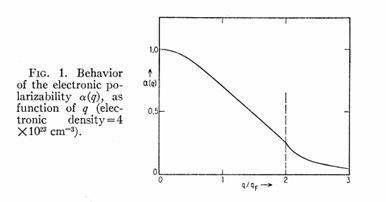
\includegraphics[height=4cm]{1.jpg}
    \end{minipage}
    \hfill
    \begin{minipage}[b]{0.49\textwidth}
    \centering
    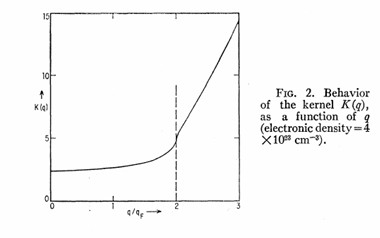
\includegraphics[height=4cm]{2.jpg}
    \end{minipage}
\end{figure}
\section{The Slowly Varying Density Gas}
The slowly varying density gas is studied to describe electronic systems in which the electron density changes gradually in space. This approach is fundamental in condensed matter physics and quantum chemistry, as many real systems, such as atoms, molecules, and solids, exhibit electron densities that are not uniform, but whose variations are smooth enough to be treated with theoretical approximations. This is addressed in the theoretical study of an electron gas whose density varies smoothly in space. This analysis is framed within the density functional theory and aims to extend traditional approximations, such as the Thomas-Fermi method, to describe more complex electronic systems. Below is a generalized summary of the main objectives and results of each subsection, highlighting the most relevant equations.

The initial goal is to derive the Thomas-Fermi equation as a basic approximation to describe the electron gas. For this purpose, an energy functional is used, which includes terms for kinetic energy, Coulomb interaction, and external potential energy:
\begin{equation}
E[n] = \int v(r) n(r) \, dr + \frac{1}{2} \int \frac{n(r) n(r')}{|r - r'|} \, dr \, dr' + \frac{3}{10} \left( 3 \pi^2 \right)^{2/3} \int \left[ n(r) \right]^{5/3} \, dr
\end{equation}
Minimizing this functional under the constraint of particle number conservation
\begin{equation}
\delta \left[ E_v[n] - u \int n(r) \, dr \right] = 0
\end{equation}
yields a differential equation
\begin{equation}
v(r) + \int \frac{n(r) n(r')}{|r' - r|} \, dr' + \frac{1}{2} \left( 3 \pi^2 \right)^{2/3} n(r)^{2/3} - \mu = 0
\end{equation}
which relates the electron density to the external potential and the internal potential generated by electronic interactions. This equation is a fundamental tool for describing systems with slowly varying densities.

Subsequently, a gradient expansion is introduced as an improvement to the Thomas-Fermi approximation. In this approach, it is assumed that the energy functional can be expanded in terms of density gradients, allowing for more precise corrections. The general form of this expansion is expressed as
\begin{equation}
g_r[n] = g_0(n(r)) + \sum_{i=1}^{3} \left( g_i(n(r)) \nabla_i n(r) \right) + \sum_{i,j=1}^{3} \left[ g_{i,j}(n(r)) \nabla_i n(r) \nabla_j n(r) + g_{i,j}^{(2)}(n(r)) \nabla_i \nabla_j n(r) \right] + \dots
\end{equation}
where higher-order terms in the gradients are accompanied by coefficients that depend on the local density. This development is useful for describing systems with more complex density variations, although it remains a valid approximation only for smoothly varying densities.

In the analysis of the coefficients of the gradient expansion, a connection is made between these coefficients and the response properties of the uniform electron gas. In particular, electronic polarizability is used, which is expanded in powers of the wave vector:
\begin{equation}
\alpha(q) = 1 + c_2 q^2 + c_4 q^4 + \ldots
\end{equation}
The expansion coefficients, such as the second and fourth-order ones, are expressed in terms of the polarizability coefficients:
\begin{equation}
\frac{g_2}{4\pi} = \frac{1}{4} \left( - c_4 + c_2'^2 \right)
\end{equation}
and
\begin{equation}
\frac{g_2}{4\pi} = \frac{1}{2} \left( - c_6 + 2c_2 c_4 - c_2'^3 \right)
\end{equation}
This approach allows linking the properties of the uniform gas with the corrections needed to describe nonuniform systems.

To improve the accuracy of the gradient expansion, a partial sum of the terms in this expansion is proposed. This method, described as
\begin{equation}
g_r[n] = g_0(n(r)) + \int \left( K_{n(r)}(r') \left[ n\left(r + \frac{1}{2} r'\right) - n(r) \right] \cdot \left[ n\left(r - \frac{1}{2} r'\right) - n(r) \right] \right) dr' + \ldots
\end{equation}
captures more complex effects in real systems by including additional terms not present in the standard expansion. Although its practical utility has not been fully evaluated, this formulation has the potential to overcome the limitations of traditional approximations.

Finally, approximate expressions for the coefficients of the gradient expansion are presented, based on calculations for the uniform electron gas. For example, the high-density expansion for the kinetic, exchange, and correlation energy is used:
\begin{equation}
g_0(n) = \left( \frac{2.21}{r_s^2} - \frac{0.916}{r_s} + 0.062 \ln(r) - 0.096 + O(r_s) \right) n
\end{equation}
as well as expressions for electronic polarizability in different approximations, such as the random phase approximation:
\begin{equation}
\alpha(q) = \frac{2\pi}{k t^2} \left[ 1 + \frac{q^2}{k_t^2} S(q) \right]^{-1}
\end{equation}
and the one including exchange effects:
\begin{equation}
\alpha(q) = \frac{2\pi}{k_t^2} \left[ 1 + \frac{1}{2} \frac{q^2}{q^2 + k_F \left( \frac{q^2}{k_t^2} \right) S(q)} \right]^{-1}
\end{equation}
These expressions allow the quantitative evaluation of the terms in the gradient expansion for real systems, although their accuracy depends on the quality of the approximations used.

\newpage
\section{Conclusion}
In this work, we have reviewed the Density Functional Theory (DFT), beginning with the theoretical principles of Hohenberg and Kohn. We explained how this theory changed the study of complex systems by making it easier to solve quantum problems. Instead of dealing with complicated wavefunctions, DFT focuses on the electron density, which is much simpler and depends on only three spatial variables.
\section{Bibliografias}
\begin{enumerate}
    \item Feliciano Giustino. Materials modelling using density functional theory: properties and predictions. Oxford University Press, 2014.
    \item Richard M. Martin and Richard Milton Martin. Electronic structure: basic theory and practical methods. Cambridge University Press, 2004.
    \item Chávez, V. H., & Wasserman, A. (año). Towards a density functional theory of molecular fragments. What is the shape of atoms in molecules? , \\https://raccefyn.co/index.php/raccefyn/article/view/960/2734
    \item Orio, M., Pantazis, D. A., & Neese, F. (2009). Density functional theory. Journal of Computational Chemistry, 30(3), 420-435. https://doi.org/10.1007/s11120-009-9404-8
    \item Takada, S. (2011). Theory of superconductivity in graphite intercalation compounds. En P. Bhattacharya, R. Fornari & H. Kamimura (Eds.), Comprehensive Semiconductor Science and Technology (pp. 410-426). Elsevier. https://doi.org/10.1016/B978-0-44-453153-7.00131-0
\end{enumerate}
 
\end{document}
